The first layer of the backpack is the music player layer. This layer is responsible for connecting the music player to the backpack and the backpack website. The different subsystems within this layer are the music player, the website, and the Raspberry Pi. The music player system is contingent upon whatever device/player the user prefers. This is a black-box system that will not be designed by the Sound Squad team.

\subsection{Website}
The website will serve as a means of product information/instructions, possible play list creation and management, and point of sale for purchase of other Sound Squad items. The website will communicate with the music player using API calls, and communicate with the backpack through a programmed connection with the backpack's Raspberry Pi. The website will have a database subsystem for user authentication and saving user settings and playlists.

\begin{figure}[h!]
	\centering
 	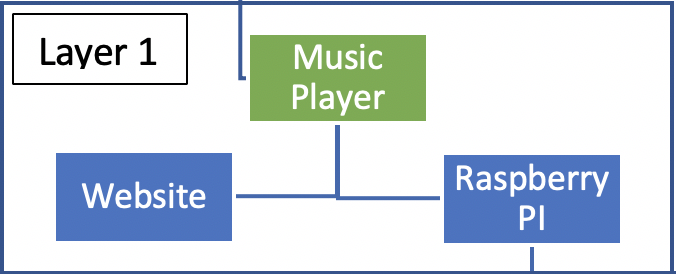
\includegraphics[width=0.60\textwidth]{images/subsystem1}
 \caption{Music player subsystem - website}
\end{figure}

\subsubsection{Assumptions}
Sound squad has made the assumption that APIs exist for all required functionality and interface between the website and the music player. Sound squad also made the assumption that users will have Wifi for the connection of the website changes to the Raspberry Pi.

\subsubsection{Responsibilities}
The website will be responsible for allowing the user to login to the Sound Squad site and connect to the music player site, make purchases of new products, create playlists and select songs to play, and finally to make advanced settings changes.

\subsubsection{Subsystem Interfaces}
The website will make an API call out to the music player and receive a rest endpoint containing the request/data. The website will connect to a Raspberry Pi via WiFi.

\begin {table}[H]
\caption {Website interfaces} 
\begin{center}
    \begin{tabular}{ | p{1cm} | p{6cm} | p{3cm} | p{3cm} |}
    \hline
    ID & Description & Inputs & Outputs \\ \hline
    \#1 & Connection to the music player & \pbox{3cm}{API call} & \pbox{3cm}{API endpoint}  \\ \hline
    \#2 & Connection to the Raspberry Pi & \pbox{3cm}{NA} & \pbox{3cm}{Music signal}  \\ \hline
    \end{tabular}
\end{center}
\end{table}

\subsection{Raspberry Pi}
The Raspberry Pi will act as the medium between the music player layer and the music filter layer. It receives and passes on any audio signals it receives. It also receives and passes on any relevant instructions from the website. The Raspberry Pi will be maintaining a WiFi connection with the website, while also receiving and sending audio signals.

\begin{figure}[h!]
	\centering
 	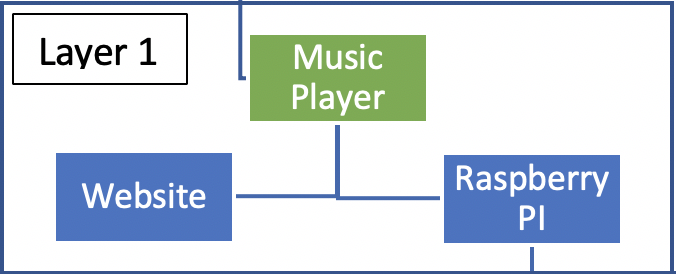
\includegraphics[width=0.60\textwidth]{images/subsystem1}
 \caption{Music player subsystem - Raspberry Pi}
\end{figure}

\subsubsection{Assumptions}
We assume that a Raspberry Pi that meets our specifications is readily available. We also assume that the Raspberry Pi will be capable of maintaining a WiFi connection, and that it will be able to efficiently receive and pass on the music signals. Finally, we assume that, if any peripheral attachments for the Raspberry Pi are needed for our system, they will also be readily available.

\subsubsection{Responsibilities}
The Raspberry Pi is responsible for maintaining a connection to the website and the music player. It needs to maintain a Wifi connection with the website. It is also the responsibility of the Raspberry Pi to forward the music signals to the pre-amp. It must also take in and pass on any user-given changes in audio settings.

\subsubsection{Subsystem Interfaces}

\begin {table}[H]
\caption {Raspberry Pi interfaces} 
\begin{center}
    \begin{tabular}{ | p{1cm} | p{6cm} | p{3cm} | p{3cm} |}
    \hline
    ID & Description & Inputs & Outputs \\ \hline
    \#1 & WiFi Connection to Website & \pbox{3cm}{ Changes on website } & \pbox{3cm}{ Raspberry Pi sends changes to appropriate system }  \\ \hline
    \#2 & Connection to the music player & \pbox{3cm}{ Music/audio signals } & \pbox{3cm}{ Music/audio signals sent to pre-amp }  \\ \hline
    \end{tabular}
\end{center}
\end{table}



